\documentclass[pdflatex,iicol,sn-mathphys-num]{sn-jnl}
\usepackage{graphicx,xurl,amsmath,amssymb,booktabs,array,tabularx,microtype,placeins,balance,tikz,capt-of}
\usetikzlibrary{arrows.meta,positioning}
\providecommand{\burl}[1]{\url{#1}}
\hypersetup{pdftitle={Adaptive Transfer Learning for Cold-Start Electric Vehicle Charging Demand Forecasting},pdfauthor={AIP491 G10 Research Team}}
\raggedbottom
\begin{document}
\title[Adaptive transfer learning]{Adaptive Transfer Learning for Cold-Start Electric Vehicle Charging Demand Forecasting}
\author{AIP491\_G10 Research Team}
\abstract{Limited target history makes it difficult to forecast demand at a charging location and to determine how strongly a transferred model should retain its source representation. We study 24-hour energy forecasting from 24 hours of observations, with initial target histories of 7, 14 and 28 days. The experiments distinguish source initialization, latent-retention regularization, retention selection and adaptive forecast fusion. Independent baseline implementations support transfer and a competitive standard GRU backbone. On twelve additional UrbanEV Development entities, source fine-tuning reduces MAE by 29.8--33.4\% relative to calibrated target-only training. Confidence-guided retention has conditional benefits: the original selector beats fixed retention in 9 of 21 historical namespace--history groups; a separate common-bank selector beats its calibrated fixed comparator at 28-day history but loses at 7 and 14 days. A later-window four-target study slightly favors discrete selection over calibrated fixed retention, while its continuous hypergradient controller is worse. A subsequent two-GRU fusion system beats single fixed retention in 18 of 21 historical groups. A matched static fusion also wins 18 groups; adaptive weighting improves on static fusion in 12 and worsens nine. These results support source transfer and complementary adaptation trajectories, while limiting the claim that adaptation of the retention decision itself consistently improves forecasting. All follow-up comparisons are exploratory and do not establish performance on an untouched test cohort.}
\keywords{EV charging, cold start, transfer learning, GRU, latent retention, confidence-guided selection, online forecasting}
\maketitle

\section{Introduction}
A charging location with little recorded history provides few complete examples for a daily forecasting model. Established locations can supply a pretrained model, but their charging patterns need not match those of a target location. Strong source retention may resist useful local adaptation; weak retention may allow a model to forget structure that remains helpful. The research question is therefore not simply whether transfer improves a forecast, but whether observed target errors can guide how source influence is used during adaptation.

We investigate this question using UrbanEV and CHARGED charging series \cite{urbanev2025,charged2025}. Cold start means a limited recorded target prefix of 7, 14 or 28 days. We simulate this restriction on existing dataset identifiers; we do not infer the physical opening date of a charging site. Each daily origin uses the previous 24 hourly bins to predict the next 24 hourly energy values. Missing history is represented explicitly, and updates require complete labels that have already arrived.

The investigation has four linked questions. First, does transfer remain useful when target-only training is given a calibrated initial training budget? Second, is GRU a reasonable compact backbone compared with classical, recurrent, convolutional, attention and spatial alternatives? Third, do fixed latent retention and confidence-guided retention selection improve on simple source fine-tuning? Fourth, can adaptive weighting of complementary source-initialized forecasters improve on a single fixed-retention model, and how much of that improvement requires changing the weights?

These questions require different controls. A comparison against target-only training tests the value of source initialization. A comparison against a tuned constant retention coefficient tests the retention decision. A comparison against a static mixture of the same expert forecasts isolates the incremental value of online weighting. Treating all three comparisons as one controller result would misidentify the source of improvement.

The empirical analysis separates confidence-guided retention, continuous-coefficient adaptation and two-expert forecast fusion. Its contributions are a controlled assessment of transfer after target-training calibration, measured fixed-coefficient sensitivity, and matched comparisons that distinguish retention decisions from forecast complementarity. The evidence includes both favorable and adverse outcomes: strong transfer gains, conditional retention-selection gains, and broader historical gains from complementary forecasts with a smaller, mixed weighting increment.

\section{Background and methodological rationale}
\subsection{Forecasting backbones}
A recurrent encoder summarizes historical sequences through a hidden state. GRU gates control the integration of the current input and the previous hidden state \cite{cho2014}. We use the standard PyTorch recurrence \cite{pytorch211}; no custom GRU layer or gate is proposed. The backbone choice keeps the retention experiments tied to one established implementation, so changes in forecast quality can be examined without simultaneously redesigning the network.

Classical lag-based predictors, tree ensembles, recurrent networks, temporal convolutions and attention provide different inductive biases. The completed baseline work includes these families rather than assuming that a recurrent model must win. The official TimeXer adapter \cite{wang2024timexer} is distinguished from a custom attention adapter because their tokenization and construction differ. A spatial GCN--LSTM uses additional support histories and therefore does not receive exactly the same information as a single-entity forecaster.

\subsection{Transfer and explicit retention}
Source initialization and explicit source regularization are different mechanisms. Initialization sets the starting model parameters. Regularization changes subsequent optimization. Work on $L^2$-SP \cite{li2018} illustrates regularization toward a pretrained parameter reference. Our implementation instead penalizes displacement of the target's latent representation from a frozen source encoder, after coordinate-wise scaling. This particular penalty and the EV replay protocol are study choices, not a consequence of that paper.

A nonzero retention coefficient can help when source features remain useful, but its effect depends on the scale of both losses and their gradients. The coefficient is not a percentage of knowledge retained. Removing the explicit penalty also does not undo transferred initialization. These distinctions matter when interpreting both the zero-retention comparator and the fast expert used later.

\subsection{Adaptive decisions and evidence}
The original controller uses paired target forecast errors and dependence-aware block resampling, motivated by the bootstrap literature \cite{kunsch1989}. A later diagnostic updates a continuous coefficient using a one-step validation hypergradient, following the broader rationale of gradient-based hyperparameter optimization \cite{luketina2016}. The two-expert extension instead applies an exponential-loss and Fixed-share update \cite{herbster1998} to forecast weights.

These are three different decision mechanisms. A bootstrap lower bound concerns a completed block of paired errors. A validation hypergradient is a local sensitivity of a forecast loss after a virtual optimizer step. An expert posterior is an algorithmic normalized weight; it is not a confidence interval for future improvement. Neither the resampling literature nor the online-learning literature establishes that these particular EV implementations will outperform fixed retention.

\section{Forecasting task and data protocol}
\subsection{Inputs, labels and missingness}
For entity $i$ and daily origin $t$, the historical tensor is $X_{i,t}\in\mathbb R^{24\times7}$. Channels are scaled hourly energy, sine and cosine of hour, sine and cosine of weekday, weekend status and an observation mask. The separate future-calendar tensor $C_{i,t}\in\mathbb R^{24\times5}$ contains the known calendar channels for the forecast day. It contains no future energy or weather measurements.

A positive energy scale $c_i$ is fitted from the permitted target prefix and is fixed during replay. Labels and model predictions are normalized for training; evaluation returns to kWh. A missing historical energy value is represented by zero together with mask zero, while an observed zero has mask one. The mask is an input feature, not an instruction that automatically suppresses the gradients of a missing historical position.

Target labels are never filled. A training or scoring example requires a complete 24-hour future label vector. Consequently 90 scheduled daily forecast origins do not guarantee 90 scored days. Missingness can also leave very few complete examples in an apparently long prefix. Initial adaptation performs zero optimizer steps when no eligible prefix examples exist, preserving the initialized model rather than creating artificial labels.

\subsection{Causal replay}
At each origin the runner processes eligible earlier label arrivals, applies any due decision, and then issues and stores the current forecast. A forecast's own labels cannot influence its issued prediction. Complete earlier arrivals are processed in availability order and then origin order. Missing or incomplete days contribute neither a partial-day error nor a model update. A replay may flush final arrivals for diagnostics after the last issued forecast; such decisions are not retroactively credited to earlier predictions.

Source pretraining and target adaptation remain within one dataset namespace. Source and target identifiers are disjoint in the prepared split. This does not certify that every identifier denotes a distinct physical site across releases or datasets. We therefore use \emph{entity} for a selected dataset identifier and reserve site-level interpretations for cases with adequate metadata.

\subsection{Experimental scopes}
\begin{table*}[t]
\centering\small
\caption{Completed studies and their comparison scopes.}\label{tab:scopes}
\begin{tabularx}{\textwidth}{@{}>{\raggedright\arraybackslash}p{.18\textwidth}>{\raggedright\arraybackslash}p{.28\textwidth}>{\raggedright\arraybackslash}p{.12\textwidth}>{\raggedright\arraybackslash}X@{}}\toprule
Study & Target sample & Prefix & Purpose and evidence window\\\midrule
Backbone benchmarks & 4 UrbanEV Development entities; two implementations & 14 days & Fixed-recipe model and initialization comparisons; independently trained Source3 backbones\\
Calibrated GRU & 4 calibration entities; 12 additional Development entities & 7 / 14 / 28 days & Source10; initial-epoch calibration and common-bank retention comparisons\\
Coefficient diagnostic & 4 previously inspected Development entities, 3 seeds & 14 days & Source10; 28 scheduled Calibration origins, 2 excluded objective days, 60 scheduled Later origins\\
Persistent coefficient & Same four entity IDs and 3 seeds & 14 days & Separate Calibration execution; promotion criterion fails; no Later execution\\
Historical comparison & 30 UrbanEV entities plus 10 in each of 6 CHARGED namespaces & 7 / 14 / 28 days & Original selector and later stable/fast fusion; previously inspected historical cohort\\
\bottomrule\end{tabularx}
\end{table*}

Table~\ref{tab:scopes} defines the denominator for every result. The four benchmark/calibration entities are 1405, 2152, 1153 and 1693. At 14 days they have 4, 12, 13 and 13 complete prefix examples. Both baseline implementations have 65,888 eligible Source examples, but train their own neural Source models for three epochs.

The twelve additional Development entities are 1691, 2564, 2398, 1114, 1225, 1169, 1885, 1802, 2035, 1836, 1303 and 1325, selected across four prefix zero-fraction strata. Each history budget supplies 888 scored entity-days per seed, with 51--90 complete scored days per entity. These entities evaluate calibrated recipes; they are not the full historical cohort.

The historical cohort includes UrbanEV/SZH and CHARGED/AMS, JHB, LOA, MEL, SPO and SZH. Seven namespaces, three histories and seeds 42, 43 and 44 yield 21 namespace--history groups and $90\times3\times3=810$ units. There are seven namespace-specific Source models per seed, or 21 Source checkpoints; target models are then adapted separately for each entity/history/seed. UrbanEV entity 2193 remains unscored in all nine units. Coverage is 67,293 scored daily vectors per compared mixture arm, with nine null units retained explicitly.

The original cohort was called Final in the historical execution. Reusing it after inspecting results does not create another untouched test set. The follow-up results in this report are exploratory. Later is a named chronological objective in the four-target diagnostic, not a synonym for an independent test cohort.

\section{GRU forecast model and loss}
\subsection{Architecture and latent state}
The encoder has two GRU layers with hidden width 64 and zero dropout. Using within-window step $\tau$, the recurrence is
\begingroup\small
\begin{equation}\begin{aligned}
r_\tau&=\sigma(W_{ir}x_\tau+b_{ir}+W_{hr}h_{\tau-1}+b_{hr}),\\
z_\tau&=\sigma(W_{iz}x_\tau+b_{iz}+W_{hz}h_{\tau-1}+b_{hz}),
\end{aligned}\label{eq:gates}\end{equation}
\endgroup
\begin{equation}\begin{aligned}
n_\tau&=\tanh\!\left(W_{in}x_\tau+b_{in}\right.\\
&\qquad\left.+r_\tau\odot(W_{hn}h_{\tau-1}+b_{hn})\right),\\
h_\tau&=(1-z_\tau)\odot n_\tau+z_\tau\odot h_{\tau-1}.
\end{aligned}\label{eq:hidden}\end{equation}
These are the PyTorch gate conventions \cite{pytorch211}; in particular, the reset gate is applied after the recurrent affine transformation in the candidate state. Hidden state is reset for each input window and is not passed between entities.

The last-layer final state $h_{24}\in\mathbb R^{64}$ is concatenated with the 120 flattened future-calendar values. The head applies a width-64 linear layer, ReLU, a 24-output linear layer and Softplus. The primary forecaster has 52,376 trainable parameters. A same-width, two-layer LSTM with this head would have 65,368; this is a parameter-count comparison, not a measured speed or accuracy advantage.

\subsection{Forecast loss and latent retention}
Let $B$ be a batch of complete examples for one target, and let $\widetilde y$ and $\widehat{\widetilde y}$ denote normalized labels and predictions. Forecast training uses
\begin{equation}
F_B(\theta)=\frac{1}{24|B|}\sum_{j\in B}\sum_{q=1}^{24}
\left|\widehat{\widetilde y}_{j,q}(\theta)-\widetilde y_{j,q}\right|.
\label{eq:forecastloss}\end{equation}
Let $h(x;\theta_s)$ be the frozen Source encoder output and $s_k$ the population standard deviation of its $k$th latent coordinate on the permitted Source training population. The retention term is
\begin{equation}\begin{aligned}
R_B(\theta)&=\frac{1}{64|B|}\sum_{j\in B}\sum_{k=1}^{64}u_{j,k}^{2},\\
u_{j,k}&=\frac{h_k(x_j;\theta)-h_k(x_j;\theta_s)}{s_k+\epsilon_R}.
\end{aligned}\label{eq:retention}\end{equation}
with $\epsilon_R=0.001$. The reference and scales receive no target gradients. Division occurs before squaring. The total target objective is
\begin{equation}
L_B(\theta,\lambda)=F_B(\theta)+\lambda R_B(\theta).
\label{eq:total}\end{equation}
Lambda controls an explicit representation penalty; it is neither the optimizer learning rate nor a percentage of retained knowledge. Setting lambda to zero removes the penalty while preserving transferred initialization.


Here $h(x;\theta)$ is a model output: the final hidden state of the last GRU layer. It is neither a raw observation nor a target label. Future-calendar features are concatenated after historical encoding; the retention term constrains the historical encoder representation, not the complete calendar-aware prediction head.

\subsection{Optimization meaning}
For the absolute forecast loss, the derivative with respect to a nonzero prediction residual is its sign, divided by the number of averaged elements. At zero the loss is nonsmooth; the implemented automatic differentiation uses the zero subgradient. Standard backpropagation then propagates this signal through the Softplus head and GRU. No differentiability of a discrete retention decision is required for training its candidate models.

In the retention term, division by $s_k+0.001$ occurs before squaring. Small-scale latent coordinates can therefore contribute strongly to the penalty. The source parameters and population standard deviations are frozen; only target parameters receive the target update. Forecast error and retention displacement are different quantities, so selecting a coefficient by minimizing $F+\lambda R$ across different coefficients would not be a valid forecasting comparison. Calibration selects by forecast MAE alone.

\section{Fixed retention and coefficient calibration}
\subsection{Historical fixed recipes}
Historical fixed retention uses a constant $\lambda=1$. The original selector considers $\{0,0.1,1\}$ and starts from a common target adaptation at $\lambda=0.1$. These are the executed historical settings. They are not presented as three universal weak, medium and strong knowledge-retention percentages.

The twelve-entity Development study uses independent trajectories at the same three coefficients but selects its Fixed comparator on the four calibration entities. It selects $\lambda=1,1,0$ for 7-, 14- and 28-day prefixes. Thus its Fixed row is not identical to the historical fixed-one recipe. A zero coefficient in that row still retains Source initialization.

\subsection{Expanded fixed-coefficient diagnostic}
The four-target coefficient study evaluates 21 real coefficients, including zero, using a finite Gaussian-process/expected-improvement search on positive log coefficients plus a coverage sensitivity grid. Acquisition is maximized approximately on 4,097 numeric grid points. Calibration averages forecast MAE equally across entities and paired seeds on the first 28 scheduled origins:
\begin{equation}
\lambda^*=\underset{\lambda\in\Lambda_{\rm measured}}{\operatorname{argmin}}\;
\frac{1}{4}\sum_{i=1}^4\frac{1}{3}\sum_{s=42}^{44}
\operatorname{MAE}^{\rm Cal}_{i,s}(\lambda).
\label{eq:fixedselection}
\end{equation}
The positive search interval is derived from prefix-only gradient-balance coefficients after three unregularized target epochs: its lower endpoint is 0.01 times the minimum measured balance coefficient, and its upper endpoint is 100 times the maximum. These factors deliberately span weak to dominant local penalty gradients; they are engineering coverage choices. Zero is evaluated separately. A declared upper-bound expansion rule is available, but the selected solution does not leave an unresolved boundary.

The selected value is $\lambda^*=0.798445006708$, with Calibration MAE 5.331705633 kWh versus 5.443630218 at zero. It is best among measured candidates, not a proven global optimum.

To characterize sampled behavior, the study records the local encoder-gradient ratio
\begin{equation}
\rho=\frac{\|\lambda\nabla_{\theta_{\rm enc}} R\|_2}{\|\nabla_{\theta_{\rm enc}} F\|_2+10^{-12}}.
\label{eq:ratio}
\end{equation}
Values below or above one indicate which measured gradient norm is larger locally. They do not imply that the vectors align, that their effects add constructively, or that their norm ratio determines future forecast error.

\begin{figure*}[t]
\centering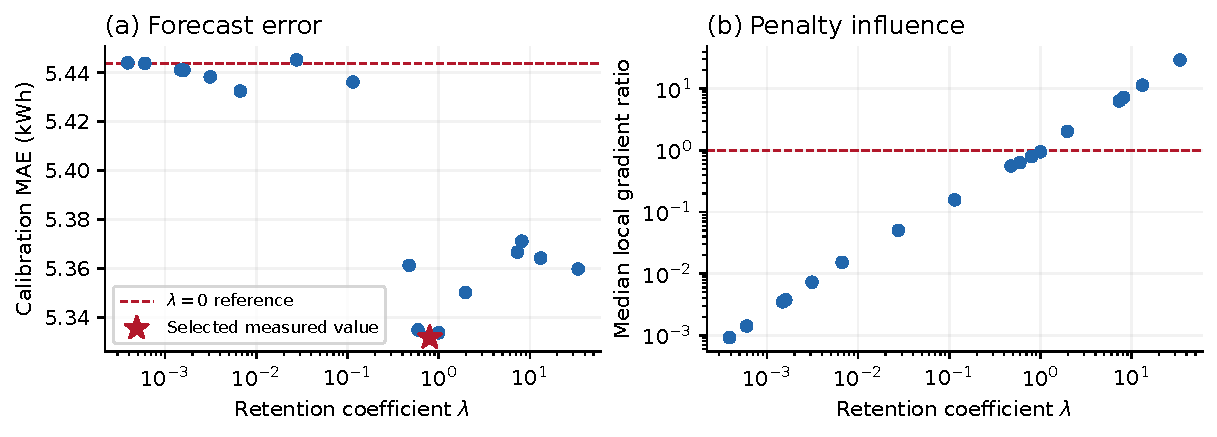
\includegraphics[width=.92\textwidth]{figures/fixed-evidence.pdf}
\caption{Measured fixed-coefficient response and local gradient ratios.}\label{fig:fixed}
\end{figure*}

Figure~\ref{fig:fixed} shows all 21 measured coefficients. Zero is displayed separately because a logarithmic axis cannot contain it. The positive domain reaches 33.8442461273. Some measured points with forecast-dominated gradients have higher Calibration error than zero; other points in that same gradient category have lower error. Retention-dominated sampled points also have lower error than zero. Thus a simple coefficient threshold does not divide useful and harmful transfer.

For example, recorded representative coefficients near 0.000390, 0.474980 and 8.163598 have median gradient ratios about 0.000922, 0.559958 and 7.234187, respectively. Their Calibration MAEs are 5.444004, 5.361266 and 5.371132 kWh. These are measured examples of distinct local behavior. They are not continuous regime boundaries, and the calibration-selected 0.798445 is kept separate from representative-point selection.

\section{Adaptive retention mechanisms}
\subsection{Confidence-gated block selection}
\begin{figure*}[t]
\centering\definecolor{FlowBlue}{HTML}{2166AC}
\definecolor{FlowRed}{HTML}{B2182B}
\begin{tikzpicture}[x=1cm,y=1cm,>=Latex,every node/.style={font=\footnotesize,align=center},
box/.style={draw=black!40,rounded corners=2pt,fill=white,inner sep=6pt,text width=3.5cm,minimum height=1.1cm},
flow/.style={->,draw=black!65,line width=.7pt}]
\node[box,fill=FlowBlue!7,draw=FlowBlue!65] (start) at (0,0) {\textbf{Selected trained state}\\Model and Adam moments};
\node[box,fill=FlowBlue!7,draw=FlowBlue!65] (fork) at (5.2,0) {\textbf{Clone at block start}\\$\lambda\in\{0,0.1,1\}$};
\node[box] (pred) at (10.4,0) {\textbf{Predict and learn}\\Three causal branches};
\node[box] (labels) at (10.4,-2.1) {\textbf{Complete arrived errors}\\Paired within the 14-day block};
\node[box,fill=FlowRed!6,draw=FlowRed!65] (decision) at (5.2,-2.1) {\textbf{Bootstrap lower bounds}\\Switch only if $L_c>0$};
\node[box,fill=FlowBlue!7,draw=FlowBlue!65] (carry) at (0,-2.1) {\textbf{Carry selected branch}\\Keep its trained model and Adam};
\draw[flow] (start)--(fork);\draw[flow] (fork)--(pred);\draw[flow] (pred)--(labels);
\draw[flow] (labels)--(decision);\draw[flow] (decision)--(carry);\draw[flow] (carry)--(start);
\end{tikzpicture}

\caption{Confidence-guided retention and trained-state continuation.}\label{fig:retention}
\end{figure*}
Figure~\ref{fig:retention} shows the original retention controller. It begins each 14-day block by cloning the selected model and Adam state into three branches, one per retention coefficient. All branches forecast causally and train on the same eligible data. Only the active branch supplies the deployed forecast. At the next boundary, complete arrived daily errors within the block are paired.

For challenger $c$ against active branch $a$, define
\begin{equation}\begin{aligned}
D_{c,d}&=e_{a,d}-e_{c,d},\\
L_c&=Q_{0.025}\!\left(\overline{D}_{c}^{*(1)},\ldots,
\overline{D}_{c}^{*(2000)}\right).
\end{aligned}\label{eq:lcb}\end{equation}
Positive differences favor the challenger. Resamples concatenate noncircular overlapping segments of three chronological valid daily observations, trimming to the original valid-day count. Both challengers use identical sampled indices. The 0.025 tail implements the specified two-challenger adjustment with interval parameter 0.05. Quantiles are linearly interpolated.

If fewer than seven complete days are available, or no challenger has $L_c>0$, the active branch is retained. Otherwise the controller selects the greatest qualifying lower bound, breaking exact ties by proximity to the current coefficient and then ascending coefficient order. The selected \emph{trained} model and optimizer continue forward, and are cloned again at the new block start. Keeping the active branch does not restore its block-start weights.

This mechanism updates a discrete retention choice and the continuation state, not the GRU architecture or Adam learning rate. The lower bound summarizes completed-block evidence; it does not guarantee a beneficial next block. Removing missing days compresses calendar gaps in the controller's valid-observation sequence. Repeated decisions, dependent samples and nonstationarity limit any confidence interpretation.

\subsection{Common-bank online selection}
The separate twelve-entity study trains independent constant-coefficient trajectories instead of reforking a chosen state every block. Its past-MAE selector and confidence selector choose outputs from this same bank, starting from the calibration-selected Fixed trajectory. The confidence variant uses seven-day blocks, at least five complete days, segment length three, 2,000 resamples and the same zero-margin principle.

This matched bank compares two output-selection rules. It is not a rerun of the original 14-day model-reforking procedure. Likewise, seven-day shadow selection over archived historical predictions does not establish what seven-day reforked training would have produced.

\subsection{Continuous validation hypergradient}
The four-target diagnostic changes a real-valued coefficient on one target branch. From current real parameters and Adam moments it creates a virtual update using two older complete arrived days $A$. A newer complete arrived day $V$, not yet used in real training, supplies forecast-only validation loss:
\begin{equation}\begin{aligned}
\widetilde\theta_t(\lambda)&=\operatorname{AdamStep}
\left(\theta_t,m_t,v_t;\nabla_\theta[F_A+\lambda R_A]\right),\\
g_t&=\left.\frac{\partial F_V(\widetilde\theta_t(\lambda))}
{\partial\lambda}\right|_{\lambda_t},\\
\lambda_{t+1}&=\Pi_{[0,U]}\left(\lambda_t-\eta_\lambda g_t\right).
\end{aligned}\label{eq:hypergradient}\end{equation}
Previous parameters and moments are fixed starting state for this local derivative. The differentiable virtual Adam step uses bias-corrected moments and does not mutate the real optimizer. After the decision, real training consumes the newly arrived example; the next forecast uses only permitted data.

Calibration selects $U=33.8442461273$, $\lambda_0=0.798445006708$, $\eta_\lambda=211.295003431$ and a cadence of one complete arrival among six declared recipes. The coefficient step size differs from the model learning rate 0.001. Adam uses betas $(0.9,0.999)$ and optimizer epsilon $10^{-8}$, separate from retention epsilon 0.001. The controller upper bound is the smallest measured coefficient above the selected Fixed value that is harmful relative to zero; if none is measured, it uses the largest finite tested coefficient. Here the fallback gives the stated upper endpoint. Step sizes are scaled from a calibration-prefix hypergradient pilot and selected across three nominal step fractions and two cadences. The projection interval is a study-specific bounded domain, not a paper-established EV constant or a measured claim that every value in it is useful.

\subsection{Persistent scalar-only follow-up}
A later Calibration execution tests a persistent shadow branch. Its candidate coefficient is restricted to a neighborhood of the calibrated Fixed anchor, approximately $[0.548445,1.048445]$, and its per-proposal coefficient change is clipped to 0.1. Acceptance requires five complete paired outcomes, mean candidate-minus-real MAE below $-0.01$ kWh, at least four wins and no paired harm above 0.05 kWh. A block expires after nine issued days without sufficient pairs.

Only an accepted scalar coefficient transfers to the real branch. Candidate weights, Adam state and RNG are not transplanted. This is different from the historical selector's trained-state continuation. Its preregistered Calibration promotion criterion determines whether a Later study proceeds; unsuccessful promotion is reported as such.

\section{Adaptive fusion of two retention experts}
\subsection{Complementary trajectories}
\begin{figure*}[t]
\centering\definecolor{FlowBlue}{HTML}{2166AC}
\definecolor{FlowRed}{HTML}{B2182B}
\begin{tikzpicture}[x=1.12cm,y=0.79cm,>=Latex,
  every node/.style={font=\footnotesize,align=center},
  box/.style={draw=black!35,rounded corners=2pt,fill=white,line width=.6pt,inner sep=7pt},
  flow/.style={->,line width=.75pt,draw=black!65},
  ref/.style={->,dashed,line width=.75pt,draw=FlowBlue}]
\node[box,text width=7.2cm,minimum height=.95cm,draw=FlowBlue!60,fill=FlowBlue!7] (source) at (7,9)
 {\textbf{Source pretraining}\\[-1pt]Established entities in one namespace $\rightarrow$ GRU checkpoint $\theta_s$ and latent scales $s$};
\node[box,text width=4.0cm,minimum height=.9cm] (input) at (7,7)
 {\textbf{Permitted target inputs}\\[-1pt]$X_t\in\mathbb R^{24\times7}$, $C_t\in\mathbb R^{24\times5}$};
\node[box,text width=5.0cm,minimum height=1.35cm,draw=FlowBlue!65,fill=FlowBlue!9] (stable) at (3.8,4.7)
 {\textbf{Stable expert}\\[2pt]GRU encoder + calendar head\\$\lambda_S=1$, $L_S=F+R$\\Newly arrived day};
\node[box,text width=5.0cm,minimum height=1.35cm,draw=FlowRed!60,fill=FlowRed!7] (fast) at (10.2,4.7)
 {\textbf{Fast expert}\\[2pt]GRU encoder + calendar head\\$\lambda_F=0$, $L_F=F$\\Last 7 calendar days};
\node[box,text width=5.0cm,minimum height=.85cm,draw=FlowBlue!65,fill=FlowBlue!9] (mix) at (7,2.5)
 {\textbf{Adaptive forecast mixture}\\$\hat y_t=w_t\hat y_{S,t}+(1-w_t)\hat y_{F,t}$};
\node[font=\small] (out) at (7,.9) {\textbf{Persist the next 24-hour energy forecast}\\[-1pt]No future energy labels enter this prediction};
\draw[flow] ([xshift=-3.584cm]source.south) -- (stable.north);
\draw[flow] ([xshift=3.584cm]source.south) -- (fast.north);
\node[fill=white,font=\footnotesize,inner sep=2pt] at (3.8,7.8) {initialize};
\node[fill=white,font=\footnotesize,inner sep=2pt] at (10.2,7.8) {initialize};
\draw[flow] (input.south) -- (7,6.1) -| ([xshift=1.4cm]stable.north);
\draw[flow] (7,6.1) -| ([xshift=-1.4cm]fast.north);
\draw[ref] (source.west) -- (.5,9) -- (.5,4.7) -- (stable.west);
\node[fill=white,text width=1.1cm,font=\footnotesize,inner sep=2pt] at (.5,6.8) {frozen\\reference\\for $R$};
\draw[flow] (stable.south) -- (3.8,2.5) -- (mix.west);
\draw[flow] (fast.south) -- (10.2,2.5) -- (mix.east);
\node[fill=white,font=\footnotesize,inner sep=2pt] at (3.8,3.2) {$\hat y_{S,t}$};
\node[fill=white,font=\footnotesize,inner sep=2pt] at (10.2,3.2) {$\hat y_{F,t}$};
\draw[flow] (mix.south) -- (out.north);
\end{tikzpicture}

\caption{Stable and fast GRUs with adaptive forecast fusion.}\label{fig:model}
\end{figure*}

The fusion extension in Figure~\ref{fig:model} retains two Source10-initialized GRUs. The stable expert is the historical Fixed model: $\lambda_S=1$, three initial target epochs when complete prefix examples exist, learning rate 0.001, and one online epoch on each newly arrived complete daily example. Its authenticated recorded forecasts are reused.

The fast expert uses $\lambda_F=0$, the same three initial epochs and learning rate, and one online epoch over available complete examples in the seven calendar days ending at the arrived example's forecast origin. The window may include permitted prefix examples, contains at most seven complete daily examples, and fits one optimizer step. It never includes labels that have not arrived.

The experts differ in both retention and update memory. A gain from combining them therefore cannot be attributed solely to different coefficients. Both start from Source; the fast expert is not target-only. Their coefficients remain constant throughout fusion.

\subsection{Weight update}
For stable weight $w_t$, the issued 24-hour forecast is
\begin{equation}
\hat y_{t,q}=w_t\hat y_{S,t,q}+(1-w_t)\hat y_{F,t,q}.
\label{eq:fusion}\end{equation}
When complete labels for an earlier forecast day $d$ arrive, use the saved pre-update expert forecasts to compute
\begin{equation}
\ell_{e,d}=\frac{1}{24c_i}\sum_{q=1}^{24}|\hat y_{e,d,q}-y_{d,q}|,
\quad e\in\{S,F\}.
\end{equation}
Feedback-event index $k$ is distinct from forecast-origin index $t$. The update is
\begin{equation}\begin{aligned}
p_k&=\frac{w_k\exp(-\eta\ell_{S,d})}
{w_k\exp(-\eta\ell_{S,d})+(1-w_k)\exp(-\eta\ell_{F,d})},\\
w_{k+1}&=(1-\alpha)p_k+\alpha(1-p_k)\\
&=\alpha+(1-2\alpha)p_k.
\end{aligned}\label{eq:fixedshare}\end{equation}
The implementation uses equivalent log-odds arithmetic. Calibration selects $w_0=0.4307815378871372$, $\eta=0.1$ and $\alpha=0.1$. Updated weights consequently lie in $[0.1,0.9]$. This bound follows from sharing, not from a lambda search. No complete feedback means no weight update; elapsed time alone does not decay the weight.

\begin{figure*}[t]
\centering\definecolor{FlowBlue}{HTML}{2166AC}
\definecolor{FlowRed}{HTML}{B2182B}
\begin{tikzpicture}[x=1.10cm,y=.95cm,>=Latex,
  every node/.style={font=\footnotesize,align=center},
  box/.style={draw=black!35,rounded corners=2pt,fill=white,line width=.6pt,inner sep=6pt,text width=3.1cm,minimum height=1.1cm},
  flow/.style={->,line width=.75pt,draw=black!65}]
\node[box,draw=FlowRed!55,fill=FlowRed!7] (labels) at (1.5,2.8) {\textbf{Arrived labels}\\Complete earlier day $d$};
\node[box,draw=FlowBlue!55,fill=FlowBlue!5] (saved) at (1.5,.4) {\textbf{Saved forecasts}\\$\hat y_{S,d},\hat y_{F,d}$\\Issued before $y_d$};
\node[box] (train) at (5.3,2.8) {\textbf{Expert updates}\\Stable: one new day\\Fast: recent window};
\node[box,draw=FlowRed!45,fill=FlowRed!4] (loss) at (5.3,.4) {\textbf{Expert losses}\\Normalized daily MAE\\$\ell_{S,d},\ell_{F,d}$};
\node[box,draw=FlowBlue!65,fill=FlowBlue!9] (weights) at (9,.4) {\textbf{Weight update}\\Posterior $p_k$\\Fixed-share $w_{k+1}$};
\node[box,draw=FlowBlue!65,fill=FlowBlue!9] (next) at (12.7,2.8) {\textbf{Current forecast}\\Updated models and $w$\\After eligible feedback};
\draw[flow] (labels.east) -- (train.west);
\draw[flow] (labels.south) -- (1.5,1.55) -- (5.3,1.55) -- (loss.north);
\draw[flow] (saved.east) -- (loss.west);
\draw[flow] (loss.east) -- (weights.west);
\draw[flow] (train.east) -- (next.west);
\draw[flow] (weights.east) -- (12.7,.4) -- (next.south);
\end{tikzpicture}

\caption{Delayed feedback for expert training and weighting.}\label{fig:feedback}
\end{figure*}

Figure~\ref{fig:feedback} separates model training from loss feedback. Expert losses refer to forecasts issued before the labels, even though the expert models also learn from the newly eligible observations. The current origin is forecast only after eligible earlier feedback has been processed.

This controller adjusts $w$, not $\lambda$. It has no bootstrap acceptance gate. Mixing two nonlinear predictors is not equivalent to training one model at coefficient $w$, and a normalized exponential weight is not confidence evidence of future benefit. Fixed-share is an established online-learning rule \cite{herbster1998}; its original guarantees are not claimed here for these unbounded energy losses and adapting GRUs.

\subsection{Calibration and matched fusion controls}
Four calibration entities and seeds 42--44 compare fast windows of 3, 7 and 14 days with learning rates 0.001 and 0.003. For each pair, a static stable weight minimizes equal-cell Calibration MAE on $[0,1]$ via the weighted-median solution of the convex absolute-error objective. This selects the seven-day, 0.001 recipe and the initial weight above.

Nine weight-controller candidates cross $\eta\in\{0.1,1,10\}$ and $\alpha\in\{0.001,0.01,0.1\}$. Calibration selects the final settings before their historical full-scope comparison. The same recipe is carried to all namespaces and histories without per-namespace recalibration. These bounded engineering grids do not establish global optimality.

The decisive control is static fusion with the same stable and fast forecasts and fixed $w_0$. Fast-only tests one component. Equal 50/50 fusion and loss-free sharing are posthoc diagnostics; in loss-free sharing, the posterior equals the prior before the same share step. This retains attraction toward one-half while removing the expert-loss signal.

\section{Experimental design and metrics}
\subsection{Baseline and training-budget controls}
Each independent baseline implementation contains 172 unique model--mode--entity--seed records: 160 nonspatial and 12 spatial. Deterministic methods are not duplicated with artificial seed replicates. Neural Source pretraining uses three epochs. Target adaptation uses three epochs, batch size four and learning rate 0.0005, followed by one online epoch per eligible arrival. The two implementations are reported separately.

The subsequent GRU study reuses Source epoch 10 and calibrates initial target epochs over $\{3,10,30,100,300\}$. The objective uses the first 28 scheduled origins of the four calibration entities, with equal entity and seed weights. The declared extension to 900 epochs is unused because no 300-epoch candidate wins. Target-only selects 30/100/100 epochs across 7/14/28 days; Source-initialized models select 3/3/10. The learning rate is 0.001. The twelve additional entities then evaluate these recipes.

\subsection{Four-target chronological objectives}
The fixed/continuous diagnostic replays all 90 scheduled origins. The first 28 define Calibration, the next two are excluded from both score objectives, and the last 60 define Later. The two excluded objective days still belong to causal replay; they are not a claim that online model training stops. Actual Later scored-day counts are 60, 22, 22 and 22 across the four entities.

The legacy discrete comparator retains its historical three-branch recipe rather than receiving matched continuous-controller tuning. It therefore uses more compute and different initialization than a single-branch constant-coefficient method. The Later outcome is a useful recorded comparator but does not isolate controller choice at equal training and search budgets.

\subsection{Aggregation and interpretation}
For scored origins $\mathcal D_{i,s}$, unit MAE is
\begin{equation}
M_{i,s}=\frac{1}{24|\mathcal D_{i,s}|}
\sum_{d\in\mathcal D_{i,s}}\sum_{q=1}^{24}
|\hat y_{i,s,d,q}-y_{i,d,q}|.
\label{eq:mae}\end{equation}
A group first averages seeds within an entity and then averages scored entities equally. All compared arms share scored origins within a unit. An unscored entity is null, not zero. We do not pool all hourly errors across unequal entities or average kWh means across namespaces with different demand scales.

For candidate $B$ and named reference $A$, percentage reduction is $100(M_A-M_B)/M_A$. Positive reductions favor the candidate. Best displayed MAEs are bold within the stated comparison; displayed ties receive equal emphasis. Group win counts are descriptive. The 21 groups reuse entities and dates across history budgets and are not 21 independent trials.

\section{Results: transfer and backbone choice}
\begin{table*}[t]
\centering\small
\caption{Independent baseline MAE (kWh; lower is better).}\label{tab:baselines}
\begin{tabular*}{\textwidth}{@{\extracolsep{\fill}}lrrrr@{}}\toprule
& \multicolumn{2}{c}{Implementation A} & \multicolumn{2}{c}{Implementation B}\\\cmidrule(lr){2-3}\cmidrule(l){4-5}
Model & Target only & Transfer & Target only & Transfer\\\midrule
Daily naive & 7.0763 & -- & 7.0757 & --\\
Weekly naive & 8.4631 & -- & 8.4631 & --\\
Ridge & 5.9339 & -- & 5.9339 & --\\
SARIMA & 6.5799 & -- & 6.6771 & --\\
Random forest & \textbf{5.8008} & -- & \textbf{5.8204} & --\\
XGBoost & 6.4847 & -- & 6.4613 & --\\
MLP & 8.6711 & 5.5196 & 8.6855 & 5.4753\\
GRU & 8.9406 & \textbf{5.3150} & 8.9239 & 5.3157\\
LSTM & 8.9360 & 5.3356 & 8.9565 & 5.3168\\
TCN & 8.0734 & 5.3447 & 7.8415 & 5.3027\\
Custom attention & 8.1209 & 5.5823 & -- & --\\
Official TimeXer & -- & -- & 7.0224 & \textbf{5.1979}\\
GCN--LSTM (spatial) & 7.1288 & -- & 7.1790 & --\\
\bottomrule\end{tabular*}
\end{table*}

Table~\ref{tab:baselines} compares model families within each implementation and training mode. A dash denotes an unreported mode, not zero error. Spatial support histories make GCN--LSTM a supplementary information-set comparison.

All 60 paired neural entity--seed comparisons in each implementation favor Source initialization. Implementation A's transferred GRU is lowest at 5.3150 kWh, compared with LSTM 5.3356 and TCN 5.3447. In implementation B, official TimeXer is lowest at 5.1979, ahead of TCN 5.3027 and GRU 5.3157. The custom attention model in A is not a matched replication of official TimeXer in B.

GRU is therefore a competitive, compact controlled backbone, not the universally best architecture. Its 52,376 parameters are fewer than the 65,368 of a same-width two-layer LSTM with the same head. This parameter count does not establish an observed runtime advantage. These small fixed-recipe benchmarks also do not provide an exhaustive hyperparameter-optimized model ranking.

\begin{figure*}[t]
\centering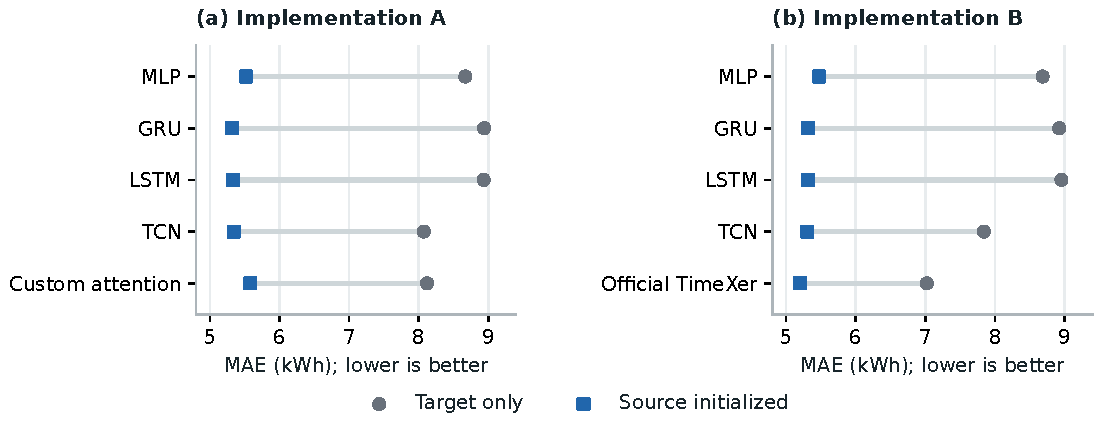
\includegraphics[width=.9\textwidth]{figures/backbones.pdf}
\caption{Paired initialization results for neural backbones.}\label{fig:backbones}
\end{figure*}

\begin{table}[t]
\centering\small
\caption{Calibrated GRU: twelve-entity Development MAE.}\label{tab:dev}
\begin{tabularx}{\columnwidth}{@{}Xrrr@{}}\toprule
Method & 7 days & 14 days & 28 days\\\midrule
Daily naive & 5.0906 & 5.0906 & 5.0906\\
Weekly naive & 6.0773 & 6.0773 & 6.0773\\
Target only & 5.0521 & 4.8341 & 4.7697\\
Source fine-tune & 3.3671 & 3.3046 & 3.3482\\
Fixed (bank) & \textbf{3.3186} & \textbf{3.2670} & 3.3482\\
Past MAE (bank) & 3.3234 & 3.2904 & 3.3252\\
Confidence (bank) & 3.3234 & 3.2755 & \textbf{3.3140}\\
\bottomrule\end{tabularx}
\end{table}

After calibrating initial training, source fine-tuning remains below target-only by 33.35\%, 31.64\% and 29.80\% at 7, 14 and 28 days (Table~\ref{tab:dev}). This supports source initialization under the tested short-history setting. Absolute errors are not compared directly with the Source3 backbone benchmark because its cohort and training recipe differ.

The retention increment is smaller. Calibrated Fixed is lowest at seven and fourteen days; the common-bank confidence selector is lowest at twenty-eight days. At 28 days its 3.313967 kWh is 1.02\% below the calibrated Fixed row, which selected zero retention. A retrospectively chosen constant-one trajectory scores 3.292501, below the confidence selector. That retrospective choice uses evaluated outcomes and is not a deployable replacement for calibration selection. Together these results show conditional selection benefits rather than consistent dominance.

\section{Results: retention adaptation}
\begin{table}[t]
\centering\small
\caption{Four-target registered Later objective (kWh).}\label{tab:later}
\begin{tabularx}{\columnwidth}{@{}Xrr@{}}\toprule
Method & MAE & $\Delta$ vs Fixed\\\midrule
Transfer, $\lambda=0$ & 4.8686 & +0.065543\\
Calibrated Fixed & 4.8031 & +0.000000\\
Legacy discrete selector & \textbf{4.7983} & -0.004795\\
Continuous hypergradient & 4.8062 & +0.003169\\
Frozen $\lambda$ control & 4.8031 & +0.000000\\
\bottomrule\end{tabularx}
\end{table}

The discrete comparator has the lowest recorded Later mean, 4.798259 versus calibrated Fixed 4.803054 kWh (Table~\ref{tab:later}), approximately 0.100\% lower. The continuous hypergradient controller gives 4.806223, which is 0.003169 kWh worse than Fixed. Its improvements on three entity means do not override the adverse equal-entity aggregate. Frozen coefficient exactly reuses Fixed where the executable configurations match; it is not an independent retraining replicate.

The continuous controller changes coefficients, but coefficient movement alone is not evidence of forecast improvement. Recorded decision values include both zero-bound contacts and positive values above the Fixed anchor. The full-90 descriptive mean favors a different ordering because it includes Calibration and Later together. We retain the registered Later objective instead of switching to that more favorable summary.

\begin{table}[t]
\centering\small
\caption{Separate persistent-study Calibration MAE (kWh).}\label{tab:persistent}
\begin{tabularx}{\columnwidth}{@{}Xr@{}}\toprule
Method & MAE\\\midrule
Calibrated Fixed & 5.331706\\
Immediate coefficient update & \textbf{5.318962}\\
Persistent scalar-only update & 5.331587\\
\bottomrule\end{tabularx}
\end{table}

The later persistent-study Calibration is a separate execution and window (Table~\ref{tab:persistent}). Immediate and persistent updates both have favorable Calibration means relative to Fixed. Persistent improvement is only 0.000118478 kWh, below its required 0.01 kWh promotion gain, with one accepted decision out of 57 and cost 1.614 times Fixed. The promotion criterion fails and no Later matrix follows. Neither its small favorable Calibration result nor the immediate result substitutes for a successful Later comparison.

\section{Results: historical adaptive fusion}
\begin{table*}[t]
\centering\small
\caption{Historical-cohort MAE for all 21 groups (kWh).}\label{tab:cohort}
\begin{tabular*}{\textwidth}{@{\extracolsep{\fill}}lrrrrrr@{}}\toprule
Namespace & Days & Fixed $\lambda=1$ & Original selector & Fast only & Static fusion & Adaptive fusion\\\midrule
UrbanEV/SZH & 7 & \textbf{8.0400} & 8.1014 & 8.5260 & 8.1510 & 8.1111\\
UrbanEV/SZH & 14 & \textbf{7.9758} & 8.0517 & 8.3709 & 8.0361 & 8.0016\\
UrbanEV/SZH & 28 & \textbf{7.9159} & 8.0015 & 8.3353 & 7.9879 & 7.9512\\
\addlinespace[3pt]
CHARGED/AMS & 7 & 6.1483 & 6.1559 & \textbf{6.1272} & 6.1294 & 6.1310\\
CHARGED/AMS & 14 & 6.1482 & 6.1520 & \textbf{6.1281} & 6.1305 & 6.1321\\
CHARGED/AMS & 28 & 6.1482 & 6.1529 & 6.1334 & \textbf{6.1331} & 6.1343\\
\addlinespace[3pt]
CHARGED/JHB & 7 & 1.3206 & 1.3685 & 1.3231 & 1.2230 & \textbf{1.2179}\\
CHARGED/JHB & 14 & 1.3227 & 1.3604 & 1.3611 & 1.2341 & \textbf{1.2269}\\
CHARGED/JHB & 28 & 1.2919 & 1.3560 & 1.2632 & 1.1926 & \textbf{1.1924}\\
\addlinespace[3pt]
CHARGED/LOA & 7 & 1.3220 & 1.3273 & 1.3118 & 1.2807 & \textbf{1.2803}\\
CHARGED/LOA & 14 & 1.3334 & 1.3431 & 1.3272 & 1.2895 & \textbf{1.2889}\\
CHARGED/LOA & 28 & 1.3265 & 1.3271 & 1.3139 & 1.2765 & \textbf{1.2759}\\
\addlinespace[3pt]
CHARGED/MEL & 7 & 52.8482 & 52.1542 & 52.3596 & \textbf{51.6384} & 51.6443\\
CHARGED/MEL & 14 & 54.3655 & 53.0840 & 52.9679 & \textbf{52.2222} & 52.2649\\
CHARGED/MEL & 28 & 54.2423 & 53.0832 & 52.7780 & \textbf{52.1444} & 52.1934\\
\addlinespace[3pt]
CHARGED/SPO & 7 & 2.0217 & 1.9702 & 2.0017 & 1.9284 & \textbf{1.9234}\\
CHARGED/SPO & 14 & 1.9893 & 1.9414 & 1.9444 & 1.8887 & \textbf{1.8869}\\
CHARGED/SPO & 28 & 2.0256 & 1.9679 & 1.9707 & 1.9133 & \textbf{1.9126}\\
\addlinespace[3pt]
CHARGED/SZH & 7 & 91.8211 & 90.6306 & 87.3766 & \textbf{85.7026} & 85.9166\\
CHARGED/SZH & 14 & 90.8436 & 89.3300 & 86.8287 & \textbf{85.0301} & 85.1907\\
CHARGED/SZH & 28 & 90.8853 & 89.3310 & 86.3015 & \textbf{84.6675} & 84.8648\\
\bottomrule\end{tabular*}
\end{table*}

Table~\ref{tab:cohort} places the original selector, both component experts and both fusion rules in one matched historical comparison. Bold marks the best displayed mean among these five methods per row; it does not select a different evaluation cohort.

The original confidence-gated retention selector is below fixed-one retention in 9 of 21 groups, while Fixed is lower in twelve. Its favorable namespace-level results occur in CHARGED/MEL, SPO and SZH. In the original report, all 18 finite exploratory intervals for this contrast include zero and the three UrbanEV intervals are undefined. Favorable point estimates therefore are not evidence of established statistical superiority.

Adaptive fusion is below single Fixed in 18 of 21 groups. All eighteen CHARGED groups improve, with reductions of 0.23--7.77\%. All three UrbanEV groups worsen: approximately 0.88\%, 0.32\% and 0.45\% for 7, 14 and 28 days. The result is eighteen namespace--history wins, not eighteen cities, and not improvement at every entity or every forecast day.

Static fusion also beats single Fixed in 18 of 21 groups, while Fast-only wins sixteen. This makes the static control essential: the broader success against single Fixed is largely a property of the complementary forecast family. It cannot all be assigned to the adaptive weight update.

\begin{figure*}[t]
\centering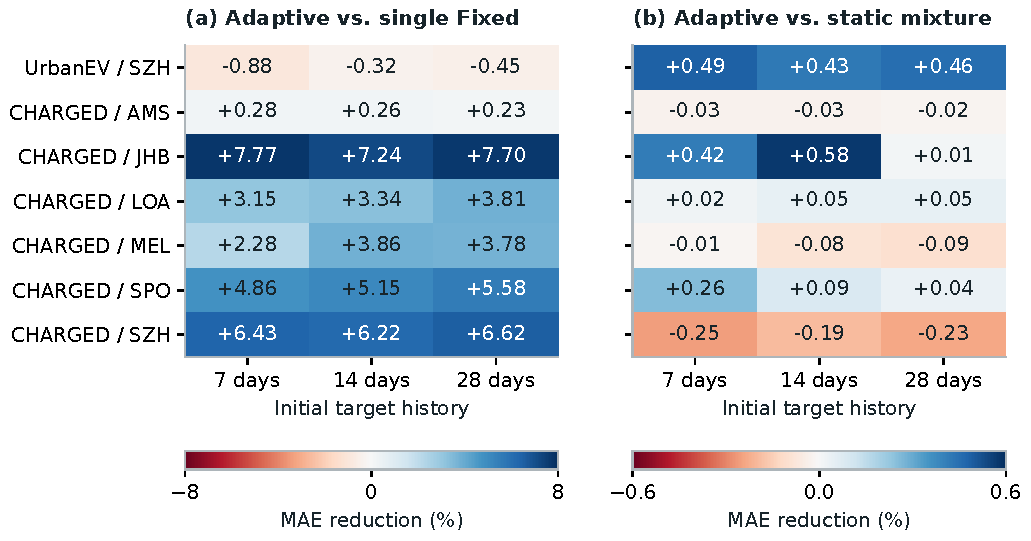
\includegraphics[width=\textwidth]{figures/cohort-comparisons.pdf}
\caption{Fusion gains against single Fixed and matched static fusion.}\label{fig:cohort}
\end{figure*}

Adaptive fusion beats matched static fusion in twelve groups and loses in nine. UrbanEV, JHB, LOA and SPO favor adaptive weights at all three histories; AMS, MEL and CHARGED/SZH favor static weights. Even where adaptive weights improve the UrbanEV mixture, the mixture remains worse than single Fixed. Figure~\ref{fig:cohort} uses separate, explicitly labeled color scales for the large family effect and the smaller weighting increment. Positive reduction is blue; adverse reduction is red.

\begin{table}[t]
\centering\small\setlength{\tabcolsep}{3pt}
\caption{Adaptive fusion versus matched fusion controls.}\label{tab:controls}
\begin{tabularx}{\columnwidth}{@{}Xrrr@{}}\toprule
Reference & Lower / 21 & Min (\%) & Max (\%)\\\midrule
Calibrated static & 12 & $-0.250$ & $+0.580$\\
Equal 50/50 & 21 & $+0.00084$ & $+0.263$\\
Loss-free sharing & 21 & $+0.00097$ & $+0.227$\\
\bottomrule\end{tabularx}
\end{table}

Against posthoc equal-weight and loss-free sharing controls, adaptive fusion is lower in all 21 group means (Table~\ref{tab:controls}). The increments are small. Their consistent signs on this inspected cohort suggest a contribution from the loss signal, but do not establish a large or statistically significant controller effect. Against calibrated static fusion, the sign remains mixed.

A separate check on the twelve additional Development entities at fourteen days gives single Fixed 3.267000, Fast-only 3.419880, static fusion 3.303021 and adaptive fusion 3.291048 kWh. Adaptive weighting improves that mixture but does not beat single Fixed. The analogous seven- and twenty-eight-day fusion cells for these twelve entities were not executed; historical-cohort values cannot fill those cells.

\section{Discussion}
\subsection{What the results establish}
The strongest repeated finding concerns source initialization. Both independent neural baseline implementations favor transfer in every paired entity--seed cell, and the calibrated twelve-entity study retains roughly 30\% improvement over target-only training. This provides a reason to study transfer for short-history targets under the tested protocol. It does not mean every source will help every new location.

The backbone evidence supports GRU as a controlled, competitive and compact implementation. It also records a stronger official TimeXer result in one implementation. Selecting GRU for the retention analysis is therefore justified by its competitiveness and manageable standard architecture, not by asserting that all alternative models lose.

For the original source-retention question, the evidence is conditional. Confidence-based selection can improve some comparisons, including the 28-day common-bank result and the four-target discrete Later result. It does not consistently improve on the relevant Fixed comparator. A local hypergradient supplies an explicit continuous update formula but does not produce a better Later aggregate in the completed study.

The fusion extension provides the broadest historical win count, but changes the mechanism. It retains both source-initialized trajectories and adjusts their forecast contribution. It cannot demonstrate that a single model has discovered the optimal source-retention coefficient or that confidence gating produced eighteen wins. Its matched static control shows how much improvement already comes from combining complementary errors.

\subsection{When source influence should be reduced}
A lower stable-expert weight means less contribution from that source-retaining forecast relative to the recent-window forecast. It is a predictor-level statement. A lower lambda means less explicit latent constraint during training. It is an optimization-level statement. Neither is a direct measurement of how much source information remains in the network.

The executed controllers use retrospective evidence to make future decisions. A completed block may be unrepresentative of the next block, and a current local validation gradient may poorly predict the next training trajectory. These mechanisms explain why plausible update rules can fail to improve a carefully calibrated constant. They are interpretations of the observed pattern, not newly verified causal explanations of each loss.

\section{Limitations and reproducibility}
The baseline sample is small, recipes are fixed rather than equally optimized, and spatial support changes the information set. The coefficient diagnostics use four previously inspected entities in one namespace. The twelve-entity study expands Development coverage but still reuses an inspected data environment. The historical mixture comparison revisits previously exposed entities and dates. None is an untouched prospective confirmation.

The units and groups are dependent. Three seeds share the same entity data; histories overlap; missingness changes scored coverage. Win counts and mean reductions do not by themselves provide confidence intervals or significance. Original bootstrap decision evidence concerns completed blocks and offers no across-block sequential safety guarantee.

Costs differ between one branch, three reforked branches, differentiable virtual updates and two continuously trained experts. The persistent follow-up records its own 1.614-fold cost, but total source pretraining, all exploration and end-to-end costs are not jointly measured across every study. Equal-cost superiority is unestablished.

Metric readbacks, file identities, matched scoring origins and model/code bindings support artifact correctness. The historical fusion audit checks 810 saved-cell hashes and independently reconstructs 66,492 consumed feedback events and 67,293 scored vectors per arm. Baseline A has an independent saved-output and label readback; baseline B reuses its published audit on unchanged ledgers. These checks do not constitute full retraining reproduction, physical issuance-time verification, reconstruction of every historical bootstrap draw, or fresh authentication of publisher raw archives.

Reproducibility materials include full-precision result ledgers, configuration locks, method implementations and saved-output verification receipts. A companion source manifest identifies the inputs to the reported tables and figures. Checkpoints and large run artifacts are retained separately from the manuscript source.

\section{Conclusion}
Transferred GRU forecasting remains competitive after stronger target-only calibration, with 29.8--33.4\% lower Development MAE from source fine-tuning. Confidence-guided retention offers conditional improvements rather than consistent superiority to Fixed; the completed continuous-coefficient study does not beat its calibrated Fixed Later result. Two-GRU adaptive fusion beats single Fixed in 18 of 21 historical groups, but static fusion does so as well. The adaptive increment wins twelve groups and loses nine, while all three UrbanEV groups still favor single Fixed. The completed evidence supports transfer and complementary adaptation trajectories, and identifies the retention decision itself as the more limited contribution requiring independent confirmation.

\FloatBarrier
\appendix
\section{Initial-training calibration}
\begin{figure*}[t]
\centering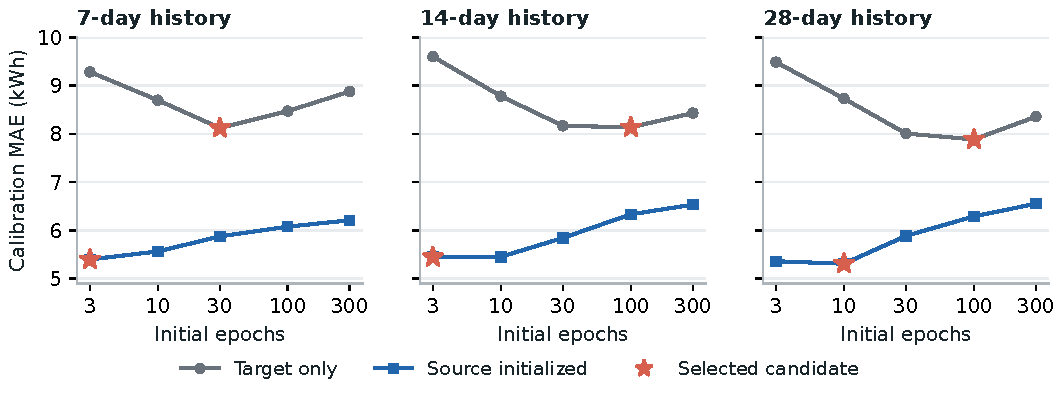
\includegraphics[width=.9\textwidth]{figures/calibration.pdf}
\caption{Calibration of the initial target training budget.}\label{fig:calibration}
\end{figure*}
Figure~\ref{fig:calibration} contains every declared initial-epoch candidate. Stars indicate selected measured candidates, not global optima. The target-only and source-initialized panels use the same MAE scale. The curves use four calibration entities; the main transfer table uses twelve additional entities. This separation prevents target-only undertraining from being used as the sole explanation for the transfer advantage.

\section{Recorded forecast-weight examples}
\begin{figure*}[t]
\centering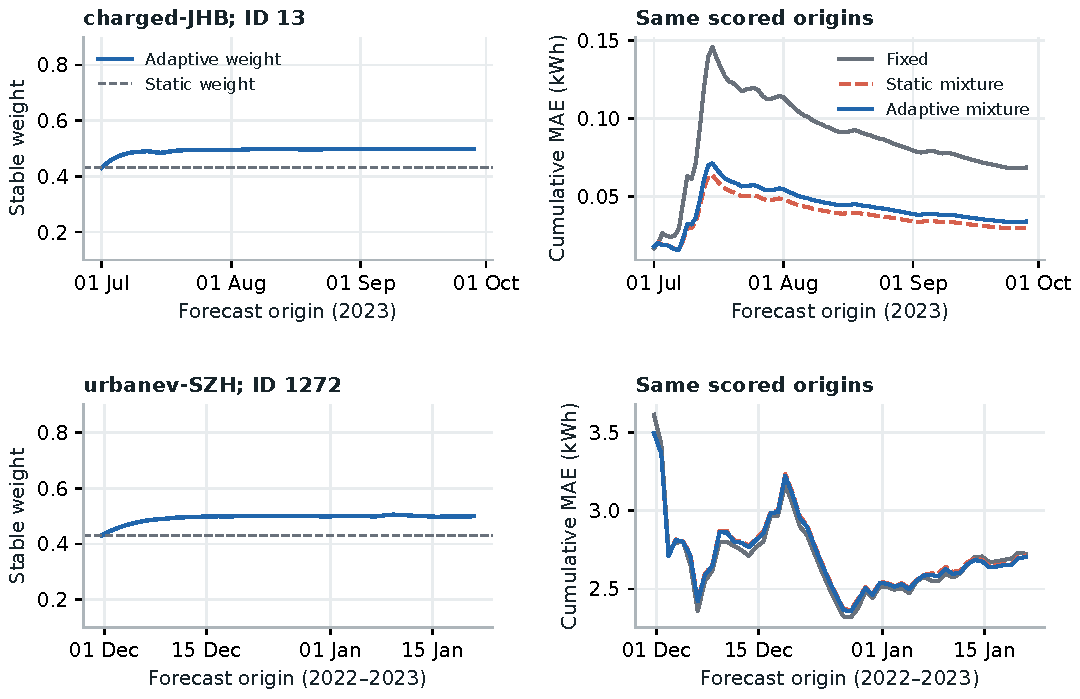
\includegraphics[width=.9\textwidth]{figures/trajectories.pdf}
\caption{Recorded weights and cumulative forecast-error contrasts.}\label{fig:traces}
\end{figure*}
The two fourteen-day-history traces use seed 42. Within JHB and UrbanEV separately, the upper median of seed-averaged percentage gain among entities with Fixed MAE above $10^{-4}$ kWh selects JHB entity 13 and UrbanEV entity 1272. This documented rule supplies a favorable and an adverse namespace example; it is not a search for the most attractive trajectory. Individual signs need not match namespace means. Dates denote forecast origins, and cumulative errors use scored origins only. Separate error axes preserve each entity's energy scale.

\FloatBarrier
\clearpage
\backmatter
\setlength{\bibsep}{0.4em}
\balance
\bibliography{references}
\end{document}
